\documentclass[tikz,border=12pt]{standalone}
\usepackage[T1]{fontenc}
\usepackage{mathpazo}
\usepackage{amsmath,amssymb}
\usetikzlibrary{arrows.meta, positioning, calc, fit, decorations.pathreplacing}

\definecolor{stblue}{HTML}{7B97AD}
\definecolor{rwgold}{HTML}{B8995E}
\definecolor{sage}{HTML}{7A9A7E}
\definecolor{dkbrown}{HTML}{3D3530}
\definecolor{wmgray}{HTML}{7B7067}
\definecolor{cream}{HTML}{F9F6F0}
\definecolor{border}{HTML}{D4C9B8}
\definecolor{terracotta}{HTML}{C47A6A}
\definecolor{lavender}{HTML}{907EA0}

\begin{document}
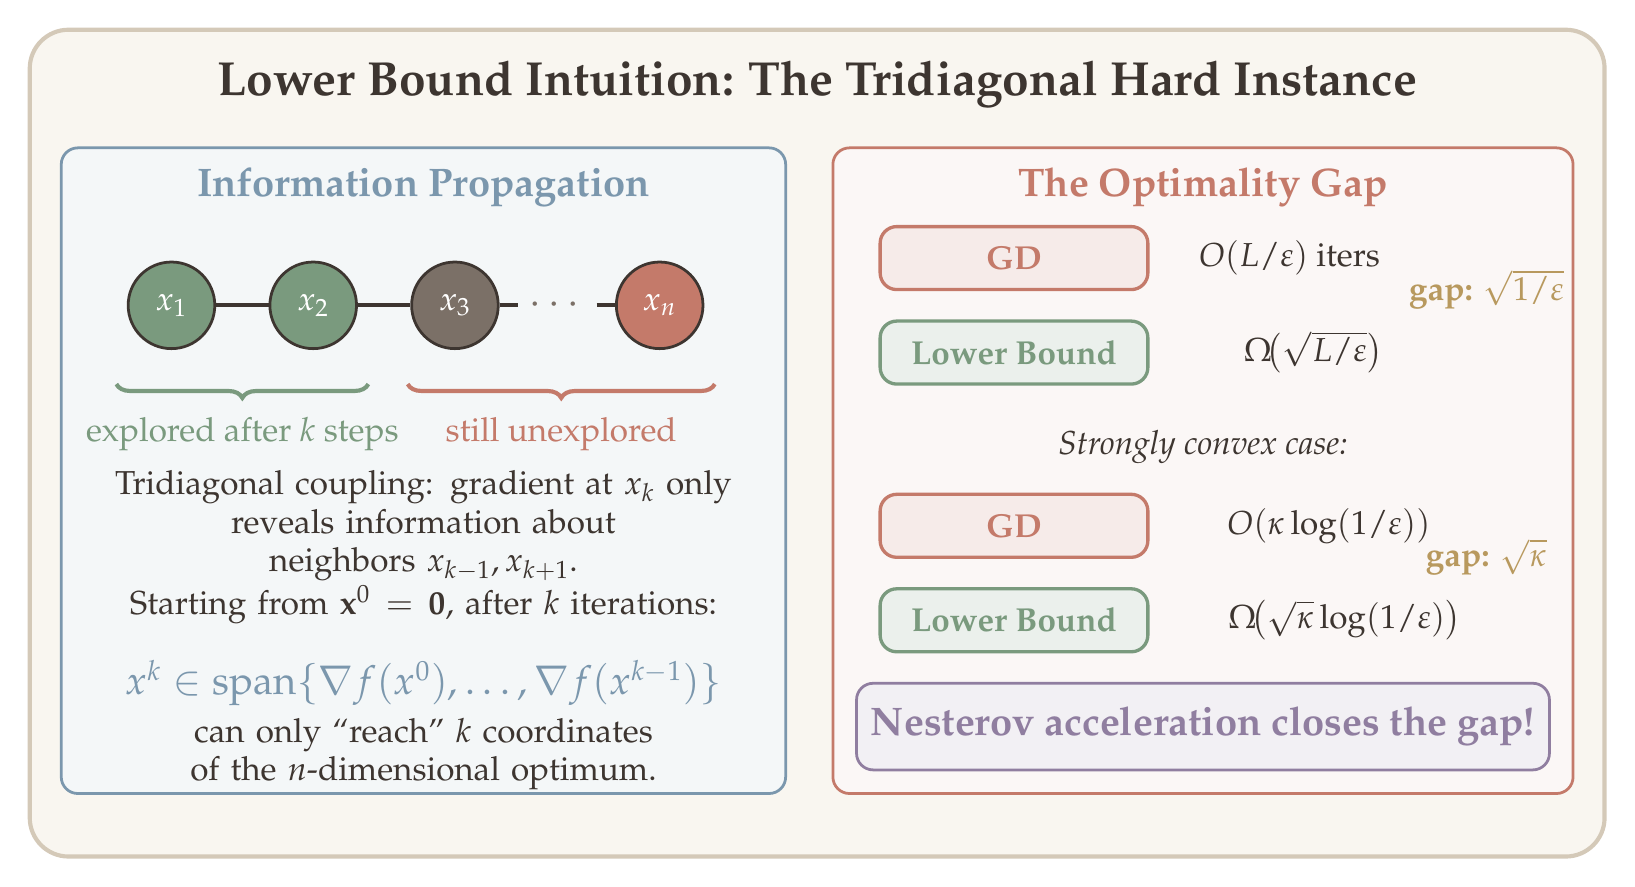
\begin{tikzpicture}[
  >={Stealth[length=4mm, width=3mm]},
  every node/.style={text=dkbrown, font=\large},
]

% Background
\fill[cream, rounded corners=14pt] (0,0) rectangle (20,10.5);
\draw[border, line width=1.5pt, rounded corners=14pt] (0,0) rectangle (20,10.5);

% Title
\node[font=\LARGE\bfseries, text=dkbrown] at (10,9.8) {Lower Bound Intuition: The Tridiagonal Hard Instance};

% --- Left panel: Information Propagation ---
\draw[stblue, line width=1pt, rounded corners=6pt, fill=stblue!8] (0.4,0.8) rectangle (9.6,9.0);
\node[font=\Large\bfseries, text=stblue] at (5,8.5) {Information Propagation};

% Chain of coordinate circles
\node[circle, draw=dkbrown, line width=1pt, fill=sage, minimum size=1.1cm, text=white, font=\large] (x1) at (1.8,7.0) {$x_1$};
\node[circle, draw=dkbrown, line width=1pt, fill=sage, minimum size=1.1cm, text=white, font=\large] (x2) at (3.6,7.0) {$x_2$};
\node[circle, draw=dkbrown, line width=1pt, fill=wmgray, minimum size=1.1cm, text=white, font=\large] (x3) at (5.4,7.0) {$x_3$};
\node[font=\Large, text=wmgray] at (6.7,7.0) {$\cdots$};
\node[circle, draw=dkbrown, line width=1pt, fill=terracotta, minimum size=1.1cm, text=white, font=\large] (xn) at (8.0,7.0) {$x_n$};

% Connections
\draw[dkbrown, line width=1.5pt] (x1) -- (x2);
\draw[dkbrown, line width=1.5pt] (x2) -- (x3);
\draw[dkbrown, line width=1.5pt] (x3) -- (6.2,7.0);
\draw[dkbrown, line width=1.5pt] (7.2,7.0) -- (xn);

% Bracket: explored
\draw[sage, line width=1.5pt, decorate, decoration={brace, mirror, amplitude=5pt}]
  (1.1,6.0) -- (4.3,6.0)
  node[midway, below=8pt, font=\large, text=sage] {explored after $k$ steps};

% Bracket: unexplored
\draw[terracotta, line width=1.5pt, decorate, decoration={brace, mirror, amplitude=5pt}]
  (4.8,6.0) -- (8.7,6.0)
  node[midway, below=8pt, font=\large, text=terracotta] {still unexplored};

% Explanation text
\node[text width=8.5cm, align=center, font=\large] at (5,4.2) {%
  Tridiagonal coupling: gradient at $x_k$ only\\
  reveals information about neighbors $x_{k-1}, x_{k+1}$.};
\node[text width=8.5cm, align=center, font=\large] at (5,3.2) {%
  Starting from $\mathbf{x}^0 = \mathbf{0}$, after $k$ iterations:};
\node[font=\Large\bfseries, text=stblue] at (5,2.2) {%
  $x^k \in \operatorname{span}\{\nabla f(x^0), \ldots, \nabla f(x^{k-1})\}$};
\node[text width=8.5cm, align=center, font=\large] at (5,1.3) {%
  can only ``reach'' $k$ coordinates of the $n$-dimensional optimum.};

% --- Right panel: The Optimality Gap ---
\draw[terracotta, line width=1pt, rounded corners=6pt, fill=terracotta!6] (10.2,0.8) rectangle (19.6,9.0);
\node[font=\Large\bfseries, text=terracotta] at (14.9,8.5) {The Optimality Gap};

% Convex case
% GD bar
\draw[terracotta, line width=1.2pt, rounded corners=6pt, fill=terracotta!15]
  (10.8,7.2) rectangle (14.2,8.0);
\node[font=\large\bfseries, text=terracotta] at (12.5,7.6) {GD};
\node[font=\large] at (16.0,7.6) {$O(L/\varepsilon)$ iters};

% Lower bound bar
\draw[sage, line width=1.2pt, rounded corners=6pt, fill=sage!15]
  (10.8,6.0) rectangle (14.2,6.8);
\node[font=\large\bfseries, text=sage] at (12.5,6.4) {Lower Bound};
\node[font=\large] at (16.3,6.4) {$\Omega\!\bigl(\sqrt{L/\varepsilon}\bigr)$};

% Gap label
\node[font=\large\bfseries, text=rwgold] at (18.5,7.2) {gap: $\sqrt{1/\varepsilon}$};

% Strongly convex case
\node[font=\large\itshape] at (14.9,5.2) {Strongly convex case:};

\draw[terracotta, line width=1.2pt, rounded corners=6pt, fill=terracotta!15]
  (10.8,3.8) rectangle (14.2,4.6);
\node[font=\large\bfseries, text=terracotta] at (12.5,4.2) {GD};
\node[font=\large] at (16.5,4.2) {$O(\kappa \log(1/\varepsilon))$};

\draw[sage, line width=1.2pt, rounded corners=6pt, fill=sage!15]
  (10.8,2.6) rectangle (14.2,3.4);
\node[font=\large\bfseries, text=sage] at (12.5,3.0) {Lower Bound};
\node[font=\large] at (16.7,3.0) {$\Omega\!\bigl(\sqrt{\kappa}\log(1/\varepsilon)\bigr)$};

% Gap label
\node[font=\large\bfseries, text=rwgold] at (18.5,3.8) {gap: $\sqrt{\kappa}$};

% Bottom conclusion box
\draw[lavender, line width=1pt, rounded corners=6pt, fill=lavender!12]
  (10.5,1.1) rectangle (19.3,2.2);
\node[font=\Large\bfseries, text=lavender] at (14.9,1.65) {Nesterov acceleration closes the gap!};

\end{tikzpicture}
\end{document}
